% V-model
\subsection{Approach}
This work has been implemented with an adaptation of V-model development process.
The original version of this process is known as a variation of the waterfall process,
with several phases dividing the beginning from the scratch and the final product,
but there is more emphasis on the coding phase.

A great feature of V-model is that every phase,
before the coding one,
has a 1:1 strong relationship with the phases that occurs after the coding,
reinforcing the mapping of the theoretical part of the project with the practical one.

The adaptation made in this project was to divide the V-model into iterations separated by the use cases.


\subsection{Use Cases}
%Sometimes it is a good idea to put domain objects in \texttt{}
%The template and the descriptions are based on the book Applying UML and Patterns: 
%An Introduction to Object-Oriented Analysis and Design and Iterative Development
%(3rd Edition) by Craig Larman.
\begin{usecase}

\addtitle{Water cycle control}{Template test} 

%Scope: the system under design
%\addfield{Scope:}{System-wide}

%Level: "user-goal" or "subfunction"
%\addfield{Level:}{User-goal}

%Primary Actor: Calls on the system to deliver its services.
\addfield{Actors:}{Microcontroller}

%Stakeholders and Interests: Who cares about this use case and what do they want?
%\additemizedfield{Stakeholders and Interests:}{
	%\item Stakeholder 1 name: his interests
	%\item Stakeholder 2 name: his interests
%}

%Preconditions: What must be true on start and worth telling the reader?
%\addfield{Preconditions:}{}
%when multiple
\additemizedfield{Preconditions:}{
    \item The Microcontroller must be installed in the system
    \item A proper relay must be installed in the system
    \item The external power supply and the water pump must be compatible
    %\item Water pump and the PWM module are working normally
} 

%Postconditions: What must be true on successful completion and worth telling the reader
\addfield{Postconditions:}
{
    The fish tank's water should be pumped to the vegetable media each quarter of an hour.
}
%when multiple
%\additemizedfield{Preconditions:}{}

%Main Success Scenario: A typical, unconditional happy path scenario of success.
\addscenario{Main Success Scenario:}{
	\item The Microcontroller executes a run cycle of 25\% in a 1 hour period.
	%\item The Microcontroller executes a run cycle of 25\% in the PWM in a 1 hour period.
	\item The circuit sends this signal to a relay.
    \item The relay activates the water pump at a 15 minutes per hour rate with the adequate voltage.
}

%Extensions: Alternate scenarios of success or failure.
%\addscenario{Extensions:}{
	%\item[2.a] Invalid login data:
		%\begin{enumerate}
		%\item[1.] System shows failure message
		%\item[2.] User returns to step 1
		%\end{enumerate}
	%\item[5.a] Invalid subsriber data:
		%\begin{enumerate}
		%\item[1.] System shows failure message
		%\item[2.] User returns to step 2 and corrects the errors
		%\end{enumerate}
%}

%Special Requirements: Related non-functional requirements.
\additemizedfield{Special Requirements:}{
	%\item R1: Operation Time Limit requirement
	\item \ref{req1}
}

% TODO: COOL Technology and Data Variations List: Varying I/O methods and data formats.
%\addscenario{Technology and Data Variations List:}{
	%\item[1a.] Alternative first action with other technology
%}

%Frequency of Occurrence: Influences investigation, testing and timing of implementation.
%\addfield{Frequency of Occurrence:}{}

%Miscellaneous: Such as open issues/questions
%\addfield{Open Issues:}{}

\end{usecase}


\subsubsection{Summary table}

\begin{table}[h]
\centering
\caption{Requirements table}
\label{tab:requirementsTable}
\begin{tabular}{|c|c|c|}
\hline
\textbf{Use Case}    & \textbf{Requirement} & \textbf{Text} \\ \hline
Optimize Water Cycle & \ref{req1}           &                 \\ \hline
\end{tabular}
\end{table}

\subsection{Requirements}

\begin{description}

\item [\req{1}]
Optimize the water cycle period between fish tank and plants medium.

\end{description}

\subsection{System Design}

\begin{figure}[h]
    \centering
    \includegraphics[width=.8\linewidth]{diagrams/systemDesign}
    \caption{A simple diagram to represent a high level design of this project}
    \label{fig:highLevelSystemDesign}
\end{figure}

\subsection{System Architecture}

\begin{figure}[h]
    \centering
    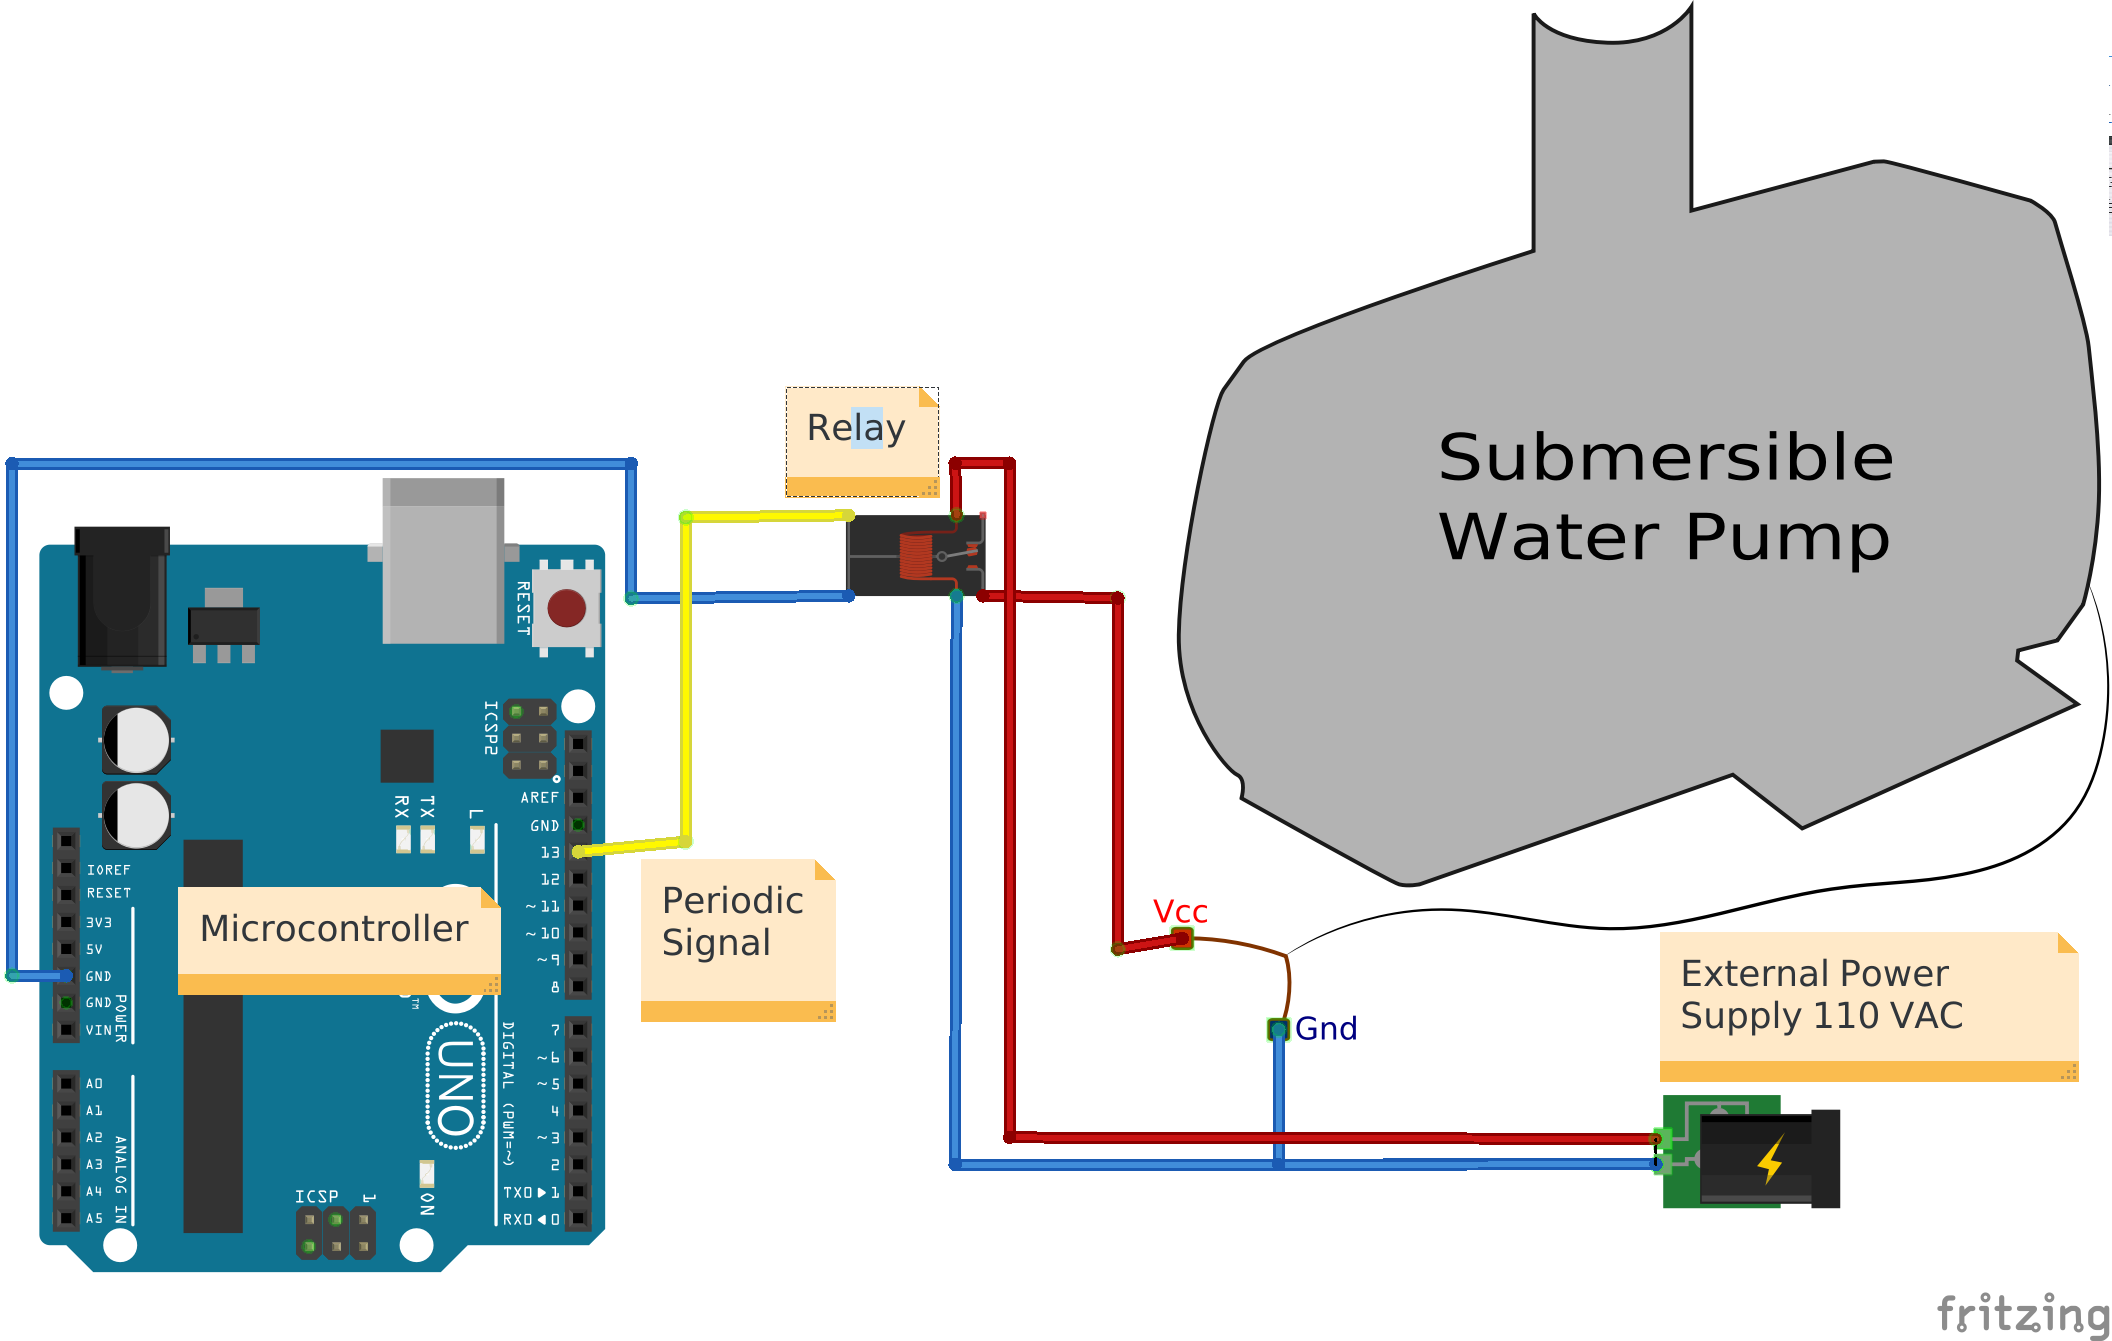
\includegraphics[width=.8\linewidth]{diagrams/architecture_bb}
    \caption{This diagram shows how the microcontroller interacts with the water pump}
    \label{fig:waterCycleDiagram}
\end{figure}

\subsection{Prototype Implementation and Project Decisions}
There are a lot of authors that have had experience with Aquaponics automation.
Most of them chooses Arduino or Raspberry Pi as the main microcontroller.

Two great reasons for the Arduino's usage are:
This work's author already has an Arduino UNO,
but not a Raspberry PI.
Besides the main reference of this work,
the \cite{Kretzinger2015},
whose author has many years of experience with Aquaponics and its automation and he uses the Arduino as microcontroller.

The chosen components have been based in the references.

% Evaluation
% Related with the requirements:
% Test 1: R1: pH Control: change constant's value and verify control work
\subsection{Results and Evaluation}
